\documentclass[a4paper]{article}
\usepackage{geometry}
\usepackage{graphicx}
\usepackage{natbib}
\usepackage{amsmath}
\usepackage{amssymb}
\usepackage{amsthm}
\usepackage{paralist}
\usepackage{epstopdf}
\usepackage{tabularx}
\usepackage{longtable}
\usepackage{multirow}
\usepackage{multicol}
\usepackage[hidelinks]{hyperref}
\usepackage{fancyvrb}
\usepackage{algorithm}
\usepackage{algorithmic}
\usepackage{float}
\usepackage{paralist}
\usepackage[svgname]{xcolor}
\usepackage{enumerate}
\usepackage{array}
\usepackage{times}
\usepackage{url}
\usepackage{fancyhdr}
\usepackage{comment}
\usepackage{environ}
\usepackage{times}
\usepackage{textcomp}
\usepackage{caption}
\usepackage{bbm}
\usepackage{enumitem}


\urlstyle{rm}

\setlength\parindent{0pt} % Removes all indentation from paragraphs
\theoremstyle{definition}
\newtheorem{definition}{Definition}[]
\newtheorem{conjecture}{Conjecture}[]
\newtheorem{example}{Example}[]
\newtheorem{theorem}{Theorem}[]
\newtheorem{lemma}{Lemma}
\newtheorem{proposition}{Proposition}
\newtheorem{corollary}{Corollary}

\floatname{algorithm}{Procedure}
\renewcommand{\algorithmicrequire}{\textbf{Input:}}
\renewcommand{\algorithmicensure}{\textbf{Output:}}
\newcommand{\abs}[1]{\lvert#1\rvert}
\newcommand{\norm}[1]{\lVert#1\rVert}
\newcommand{\RR}{\mathbb{R}}
\newcommand{\CC}{\mathbb{C}}
\newcommand{\Nat}{\mathbb{N}}
\newcommand{\br}[1]{\{#1\}}
\DeclareMathOperator*{\argmin}{arg\,min}
\DeclareMathOperator*{\argmax}{arg\,max}
\renewcommand{\qedsymbol}{$\blacksquare$}

\definecolor{dkgreen}{rgb}{0,0.6,0}
\definecolor{gray}{rgb}{0.5,0.5,0.5}
\definecolor{mauve}{rgb}{0.58,0,0.82}

\newcommand{\Var}{\mathrm{Var}}
\newcommand{\Cov}{\mathrm{Cov}}

\newcommand{\vc}[1]{\boldsymbol{#1}}
\newcommand{\xv}{\vc{x}}
\newcommand{\Sigmav}{\vc{\Sigma}}
\newcommand{\alphav}{\vc{\alpha}}
\newcommand{\muv}{\vc{\mu}}

\newcommand{\red}[1]{\textcolor{red}{#1}}

\def\x{\mathbf x}
\def\y{\mathbf y}
\def\w{\mathbf w}
\def\v{\mathbf v}
\def\E{\mathbb E}
\def\V{\mathbb V}
\def\ind{\mathbbm 1}

% TO SHOW SOLUTIONS, include following (else comment out):
\newenvironment{soln}{
    \leavevmode\color{blue}\ignorespaces
}{}


\hypersetup{
%    colorlinks,
    linkcolor={red!50!black},
    citecolor={blue!50!black},
    urlcolor={blue!80!black}
}

\geometry{
  top=1in,            % <-- you want to adjust this
  inner=1in,
  outer=1in,
  bottom=1in,
  headheight=3em,       % <-- and this
  headsep=2em,          % <-- and this
  footskip=3em,
}


\pagestyle{fancyplain}
\lhead{\fancyplain{}{Homework 4}}
\rhead{\fancyplain{}{CS 760 Machine Learning}}
\cfoot{\thepage}

\title{\textsc{Homework 4}} % Title

%%% NOTE:  Replace 'NAME HERE' etc., and delete any "\red{}" wrappers (so it won't show up as red)

\author{
\red{APOORVA KUMAR} \\
\red{908 461 5997}\\
} 

\date{}

\begin{document}

\maketitle 


\textbf{Instructions:} Use this latex file as a template to develop your homework. Submit your homework on time as a single pdf file to Canvas. Late submissions may not be accepted. Please wrap your code and upload it to a public GitHub repo, then attach the link below the instructions so that we can access it. You can choose any programming language (i.e. python, R, or MATLAB). Please check Piazza for updates about the homework.\\

\begin{soln}
    \Large
    \href{https://github.com/cybr17crwlr/ECE-760-Machine-Learning-Assignments/tree/master/Homework%204}{Homework 4 Github Link}
\end{soln}

\section{Best Prediction}
\subsection{Under 0-1 Loss (10 pts)}
Suppose the world generates a single observation $x \sim \mbox{multinomial}(\theta)$, where the parameter vector $\theta=(\theta_1, \ldots, \theta_k)$ with $\theta_i\ge 0$ and $\sum_{i=1}^k \theta_i=1$.  Note $x \in \{1, \ldots, k\}$.
You know $\theta$ and want to predict $x$. 
Call your prediction $\hat x$.  What is your expected 0-1 loss: 
$$\E[\ind_{\hat x \neq x}]$$
using the following two prediction strategies respectively?  Prove your answer.
\begin{enumerate}
    \item Strategy 1: $\hat x \in \argmax_x \theta_x$, the outcome with the highest probability.
    \begin{soln}
        \begin{align*}
            \E[\ind_{\hat x \neq x}] &= \mathbb{P}(\hat{x}\neq x)\\
            &= 1 - \mathbb{P}(\hat{x}= x)\\
            &= 1 - \mathbb{P}(x= \argmax_x \theta_x)\\
            &= 1 - \max_x \theta_x
        \end{align*}
    \end{soln}
    \item Strategy 2: You mimic the world by generating a prediction $\hat x \sim \mbox{multinomial}(\theta)$.  (Hint: your randomness and the world's randomness are independent)
    \begin{soln}
        \begin{align*}
            \E[\ind_{\hat x \neq x}] &= \mathbb{P}(\hat{x}\neq x)\\
            &= 1 - \mathbb{P}(\hat{x}= x)\\
            &= 1 - \sum_{i=1}^{i=k}\mathbb{P}(x= k)\mathbb{P}(\hat{x}= k)\\
            &= 1 - \sum_{i=1}^{i=k}\theta_i^2
        \end{align*}
    \end{soln}
\end{enumerate}

\subsection{Under Different Misclassification Losses (6 pts)}
Like in the previous question, the world generates a single observation $x \sim \mbox{multinomial}(\theta)$. Let $c_{ij} \ge 0$ denote the loss you incur, if $x=i$ but you predict $\hat x=j$, for $i,j \in \{1, \ldots, k\}$.
$c_{ii}=0$ for all $i$. This is a way to generalize different costs of false positives vs false negatives from binary classification to multi-class classification. You want to minimize your expected loss:
$$\E[c_{x \hat x}]$$
Derive your optimal prediction $\hat x$.

\begin{soln}
    We know $x$ and $\hat x$ are from independent distribution.
    \begin{align*}
        \E[c_{x \hat x}] &= \sum_{i=1}^{k}\sum_{j=1}^{k}c_{ij}\mathbb P(x=i,\hat x=j) \\
        &= \sum_{i=1}^{k}\sum_{j=1}^{k}c_{ij}\mathbb P(x=i)\mathbb P(\hat x=j)\\
        &= \sum_{i=1}^{k}\sum_{j=1}^{k}c_{ij}\theta_i\mathbb P(\hat x=j)\\
        &= \sum_{j=1}^{k}\mathbb P(\hat x=j)\sum_{i=1,i\neq j}^{k}\theta_i c_{ij}
    \end{align*}
    Now we need to choose $\hat x$ such that it minimizes $\E[c_{x \hat x}]$.
    $$
        \hat x = \argmin_{\hat x}\E[c_{x \hat x}] = \argmin_{\hat x}\sum_{j=1}^{k}\mathbb P(\hat x=j)\sum_{i=1,i\neq j}^{k}\theta_i c_{ij} \\
    $$
    Assume $\hat x=m$ where $m \in \{1, \ldots, k\}$, we get:
    $$
        \mathbb P(\hat x=j) = \begin{cases}1 & j=m\\ 0 & otherwise \end{cases}
    $$
    Therefore our equation reduces to:
    \begin{align*}
        \argmin_{\hat x}\E[c_{x \hat x}] &= \argmin_{\hat x}\sum_{j=1}^{k}\mathbb P(\hat x=j)\sum_{i=1,i\neq j}^{k}\theta_i c_{ij} \\
        &= \argmin_{m}\sum_{i=1,i\neq m}^{k}\theta_i c_{im} \\
    \end{align*}
    Thus we choose $m$, i.e. the class for $\hat x$, such that it minimizes $\sum_{i=1}^{k}\theta_i c_{im}$
\end{soln}

\section{Language Identification with Naive Bayes (8 pts each)}
Implement a character-based Naive Bayes classifier that classifies a document as English, Spanish, or Japanese - all written with 26 lower-case characters and space.

The dataset is languageID.tgz, unpack it. This dataset consists of 60 documents in English, Spanish, and Japanese. The correct class label is the first character of the filename: $y \in \{e, j, s\}$. (Note: here each file is a document in the corresponding language, and it is regarded as one data.)

We will be using a character-based multinomial Naïve Bayes model. You need to view each document as a bag of characters, including space. We have made sure that there are only 27 different types of printable characters (a to z, and space) -- there may be additional control characters such as new-line, please ignore those. Your vocabulary will be these 27 character types. (Note: not word types!)

In the following questions, you may use the additive smoothing technique to smooth categorical data, in case the estimated probability is zero. Given $N$ data samples $\{\vc{x}^{(i)}, y^{(i)}\}_{i = 1}^{N}$, where $\vc{x}^{(i)} = [x_1^{(i)}, \dots, x_j^{(i)}, \dots, x_{M_i}^{(i)}]$ is a bag of characters, $M_i$ is the total number of characters in $\vc{x}^{(i)}$, $x_{j}^{(i)} \in S, y^{(i)} \in L$ and we have $|S| = K_S, |L| = K_L$. Here $S$ is the set of all character types, and $L$ is the set of all classes of data labels. Then by the additive smoothing with parameter $\alpha$, we can estimate the conditional probability as 
$$
P_{\alpha}(a_s \mid y = c_k) = \frac{(\sum_{i = 1}^{N}\sum_{j = 1}^{M_i}\ind [x_{j}^{(i)} = a_s, y^{(i)} = c_k]) + \alpha}{(\sum_{b_s \in S}\sum_{i = 1}^{N}\sum_{j = 1}^{M_i}\ind [x_{j}^{(i)} = b_s, y^{(i)} = c_k]) + K_S \alpha},
$$
where $a_s \in S, c_k \in L$. Similarly, we can estimate the prior probability
$$
P_{\alpha}(Y = c_k) = \frac{(\sum_{i = 1}^{N}\ind [y^{(i)} = c_k]) + \alpha}{N + K_L \alpha},
$$
where $c_k \in L$ and $N$ is the number of training samples.
\begin{enumerate}
\item
Use files 0.txt to 9.txt in each language as the training data.
Estimate the prior probabilities 
$\hat p(y=e)$,
$\hat p(y=j)$,
$\hat p(y=s)$
using additive smoothing with parameter $\frac{1}{2}$. 
Give the formula for additive smoothing with parameter $\frac{1}{2}$ in this case. 
Print the prior probabilities.

\begin{soln}
The formula for additive smoothing with parameter $\alpha=\frac{1}{2}$, $K_L=|L|=3$ and $N=30$ is:
    $$
    \hat{p}(y = c_k) = \frac{(\sum_{i = 1}^{30}\ind [y^{(i)} = c_k]) + 1/2}{30 + 3/2}
    $$  
For each class we 10 samples.
    \begin{align*}
        \hat{p}(y = e) = \frac{10 + 1/2}{30 + 3/2} = \frac{1}{3} \\
        \hat{p}(y = s) = \frac{10 + 1/2}{30 + 3/2} = \frac{1}{3} \\
        \hat{p}(y = j) = \frac{10 + 1/2}{30 + 3/2} = \frac{1}{3} \\
    \end{align*}
\end{soln}

\item
Using the same training data, estimate the class conditional probability (multinomial parameter) for English
$$\theta_{i,e} := \hat p(c_i \mid y=e)$$ 
where $c_i$ is the $i$-th character. That is, $c_1 = a, \ldots, c_{26} = z, c_{27} = space$.
Again, use additive smoothing with parameter $\frac{1}{2}$.
Give the formula for additive smoothing with parameter $\frac{1}{2}$ in this case. 
Print $\theta_e$ which is a vector with 27 elements.

\begin{soln}
    The formula for additive smoothing with parameter $\alpha=\frac{1}{2}$,  $K_S=|S|=27$ and \\
    $N=\{\texttt{e0.txt, e1.txt, .., e9.txt}\}$ is:
    $$
    \theta_{i,e} = \hat p(c_i \mid y=e) = \frac{(\sum_{j\in N}\sum_{k = 1}^{M_i}\ind [x_{k}^{(j)} = c_i]) + 1/2}{(\sum_{b_s \in S}\sum_{j\in N}\sum_{k = 1}^{M_i}\ind [x_{k}^{(j)} = b_s]) + 27/2}\\
    $$
    \begin{gather*}
        \theta_{e} =    \begin{bmatrix}
                            0.06017 \\
                            0.01113 \\
                            0.02151 \\
                            0.02197 \\
                            0.10537 \\
                            0.01893 \\
                            0.01748 \\
                            0.04722 \\
                            0.05541 \\
                            0.00142 \\
                            0.00373 \\
                            0.02898 \\
                            0.02052 \\
                            0.05792 \\
                            0.06446 \\
                            0.01675 \\
                            0.00056 \\
                            0.05382 \\
                            0.06618 \\
                            0.08013 \\
                            0.02666 \\
                            0.00928 \\
                            0.0155 \\
                            0.00116 \\
                            0.01384 \\
                            0.00063 \\
                            0.17925 \\
                        \end{bmatrix}
    \end{gather*}
\end{soln}

\item
Print $\theta_j, \theta_s$, the class conditional probabilities for Japanese and Spanish.

\begin{soln}
    \begin{minipage}{0.5\textwidth}
        \begin{gather*}
            \theta_{j} =\begin{bmatrix}
                            0.13177 \\
                            0.01087 \\
                            0.00549 \\
                            0.01723 \\
                            0.0602 \\
                            0.00388 \\
                            0.01401 \\
                            0.03176 \\
                            0.09703 \\
                            0.00234 \\
                            0.05741 \\
                            0.00143 \\
                            0.0398 \\
                            0.05671 \\
                            0.09116 \\
                            0.00087 \\
                            0.0001 \\
                            0.0428 \\
                            0.04217 \\
                            0.05699 \\
                            0.07062 \\
                            0.00024 \\
                            0.01974 \\
                            3e-05 \\
                            0.01415 \\
                            0.00772 \\
                            0.12345 \\
                        \end{bmatrix}
        \end{gather*}
    \end{minipage}
    \begin{minipage}{0.5\textwidth}
        \begin{gather*}
            \theta_{s}=\begin{bmatrix}
                            0.10456 \\
                            0.00823 \\
                            0.03753 \\
                            0.03975 \\
                            0.11381 \\
                            0.0086 \\
                            0.00718 \\
                            0.00453 \\
                            0.04986 \\
                            0.00663 \\
                            0.00028 \\
                            0.05294 \\
                            0.02581 \\
                            0.05418 \\
                            0.07249 \\
                            0.02427 \\
                            0.00768 \\
                            0.0593 \\
                            0.06577 \\
                            0.03561 \\
                            0.0337 \\
                            0.00589 \\
                            9e-05 \\
                            0.0025 \\
                            0.00786 \\
                            0.00268 \\
                            0.16826 \\
            \end{bmatrix}
        \end{gather*}
    \end{minipage}
\end{soln}


\item
Treat e10.txt as a test document $x$.
Represent $x$ as a bag-of-words count vector (Hint: the vocabulary has size 27).
Print the bag-of-words vector $x$.

\begin{soln}
        $x = [164\;32\;53\;57\;311\;55\;51\;140\;140\;3\;6\;85\;64\;139\;182\;53\;3\;141\;186\;225\;65\;31\;47\;4\;38\;2\;498]$
\end{soln}

\item
For the $x$ of e10.txt, compute $\hat p(x \mid y)$ for $y=e, j, s$ under the multinomial model assumption, respectively.
Use the formula
$$\hat p(x \mid y) = \prod_{i=1}^d (\theta_{i, y})^{x_i}$$
where $x=(x_1, \ldots, x_d)$.
Show the three values: $\hat p(x \mid y=e), \hat p(x \mid y=j), \hat p(x \mid y=s)$.

Hint: you may notice that we omitted the multinomial coefficient.  This is ok for classification because it is a constant w.r.t. $y$. Also, Store all probabilities here and below in $\log()$ internally to avoid underflow. This also means you need to do arithmetic in log space. 

\begin{soln}
    Due to the underflow issue the problem was solved in the log space using the following formula. As log is an increasing function it follows the same comparison rules as the original probabilities.
    \begin{align*}
        \hat p(x \mid y) &= \prod_{i=1}^d (\theta_{i, y})^{x_i}\\
        \log(\hat p(x \mid y)) &= \sum_{i=1}^d\log((\theta_{i, y})^{x_i})\\
        \log(\hat p(x \mid y)) &= \sum_{i=1}^d x_i\log(\theta_{i, y})\\
        \hat p(x \mid y) &= e^{\sum_{i=1}^d x_i\log(\theta_{i, y})}
    \end{align*}
    Thus the condition probabilities are:
    \begin{gather*}
        \hat p(x \mid y=e) = e^{-7841.8654}\\
        \hat p(x \mid y=s) = e^{-8467.2820}\\
        \hat p(x \mid y=j) = e^{-8771.4331}
    \end{gather*}
\end{soln}

\item
For the $x$ of e10.txt, use the Bayes rule and your estimated prior and likelihood, compute the posterior $\hat p(y \mid x)$.
Show the three values: $\hat p(y=e \mid x), \hat p(y=j \mid x), \hat p(y=s \mid x)$.
Show the predicted class label of $x$.

\begin{soln}
    \begin{align*}
        \hat p(y \mid x) &= \frac{\hat p(x \mid y) \hat p(y)}{\hat p(x)} \\
        \hat p(y=e \mid x) &= \frac{\hat p(x \mid y=e) \hat p(y=e)}{\hat p(x)} = \frac{1}{3}\cdot\frac{e^{-7841.8654}}{\hat p(x)}\\
        \hat p(y=s \mid x) &= \frac{\hat p(x \mid y=s) \hat p(y=s)}{\hat p(x)} = \frac{1}{3}\cdot\frac{e^{-8467.2820}}{\hat p(x)}\\
        \hat p(y=j \mid x) &= \frac{\hat p(x \mid y=j) \hat p(y=j)}{\hat p(x)} = \frac{1}{3}\cdot\frac{e^{-8771.4331}}{\hat p(x)}
    \end{align*}
    Knowing $\hat p(x)$ is positive the predicted class is: 
    $$
    \argmax_{c_i\in\{e,s,j\}} \hat p(y=c_i \mid x) = \mathbf{e}
    $$
    Thus the predicted class for \texttt{e10.txt} is \textbf{English}
\end{soln}

\item
Evaluate the performance of your classifier on the test set (files 10.txt to 19.txt in three languages).
Present the performance using a confusion matrix. A confusion matrix summarizes the types of errors your classifier makes, as shown in the table below.   The columns are the true language a document is in, and the rows are the classified outcome of that document.  The cells are the number of test documents in that situation.  For example, the cell with row = English and column = Spanish contains the number of test documents that are really Spanish but misclassified as English by your classifier.
\begin{soln}
    \begin{center}
        \begin{tabular}{c|ccc}
            & English & Spanish & Japanese \\
            \hline
            English&10&0&0\\
            Spanish&0&10&0\\
            Japanese&0&0&10
        \end{tabular}
    \end{center}
\end{soln}


\item Take a test document.   Arbitrarily shuffle the order of its characters so that the words (and spaces) are scrambled beyond human recognition.  How does this shuffling affect your Naive Bayes classifier's prediction on this document?  Explain the key mathematical step in the Naive Bayes model that justifies your answer.

\begin{soln}
    Using \texttt{e10.txt}, we get the exact prediction of \textbf{English}. This can be attributed to the fact that the Naive Bayes technique used here only counts the number of characters in the sentence without caring about their relative position or even caring for the words they form. Thus even after shuffling them, their \textbf{representation in the model is precisely the same} as before, and we get the same output.

    The critical mathematical step which achieves this is the \textbf{calculation of conditional probability} where the probability of each feature is calculated \textbf{solely based on the class}. There is no dependence between the features themselves thus the \textbf{relative placement of characters} is \textbf{not important to the model} anymore.
\end{soln}

\end{enumerate}

\section{Simple Feed-Forward Network (20pts)}
In this exercise, you will derive, implement back-propagation for a simple neural network and compare your output with some standard library’s output. Consider the following 3-layer neural network.

\[
\hat{y} = f(x) = g(W_3\sigma(W_2\sigma(W_1x)))
\]

Suppose $x \in \mathbb{R}^d$, $W_1 \in \mathbb{R}^{d_1 \times d}$, $W_2 \in \mathbb{R}^{d_2 \times d_1}$, $W_3 \in \mathbb{R}^{k \times d_2}$ i.e. $f: \mathbb{R}^d \rightarrow \mathbb{R}^k$, Let $\sigma(z) = [\sigma(z_1), ..., \sigma(z_n)]$ for any $z \in \mathbb{R}^n$ where $\sigma(z) = \frac{1}{1 + e^{-z}}$ is the sigmoid (logistic) activation function and $g(z_i) = \frac{exp(z_i)}{\sum_{i=1}^k exp(z_i)}$ is the softmax function. Suppose the true pair is $(x, y)$ where $y \in \{0, 1\}^k$ with exactly one of the entries equal to 1, and you are working with the cross-entropy loss function given below,

\[
L(x, y) = -\sum_{i=1}^k y \text{log}(\hat{y})
\]

\begin{enumerate}
    \item Derive backpropagation updates for the above neural network. (5 pts)
    
    \begin{soln}
        Let the output of $i^{th}$ neutron in 1st layer be $a_i$, 2nd layer be $b_i$ and for the final layer be $\hat y_i$. Thus we can break down our equation as:
        \begin{align*}
            a_i &= \sigma(W_1^{i1}x_1 + W_1^{i2}x_2 + \ldots + W_1^{id}x_d) \quad \forall \; i \in \{1, \ldots, d_1\} \\
            b_i &= \sigma(W_2^{i1}a_1 + W_2^{i2}a_2 + \ldots + W_2^{id_1}a_{d_1}) \quad \forall \; i \in \{1, \ldots, d_2\} \\
            \hat y_i &= \frac{\exp{(W_3^{i1}b_1 + W_3^{i2}b_2 + \ldots + W_3^{id_2}b_{d_2})}}{\sum_{j=1}^{k}\exp{(W_3^{j1}b_1 + W_3^{j2}b_2 + \ldots + W_3^{jd_2}b_{d_2})}} \quad \forall \; i \in \{1, \ldots, k\} 
        \end{align*}

        Now for backpropagation update of weights we essentially need to calculate:
        $$
            \frac{\partial L}{\partial W_3^{ij}}, \frac{\partial L}{\partial W_2^{ij}}, \frac{\partial L}{\partial W_1^{ij}}
        $$
        Starting with the update of $W_3^{ij}$:
        $$
            \frac{\partial L}{\partial W_3^{ij}} = -\frac{\partial \sum_{m=1}^k y_m \log(\hat{y_m})}{\partial W_3^{ij}} = -\sum_{m=1}^k \frac{\partial y_m \log(\hat{y_m})}{\partial \hat y_m} \frac{\partial \hat y_m}{\partial W_3^{ij}} = -\sum_{m=1}^k \frac{y_m }{\hat y_m} \frac{\partial \hat y_m}{\partial W_3^{ij}}
        $$
        Now for $\frac{\partial \hat y_m}{\partial W_3^{ij}}$ we have two cases:\\
        Case 1: $m=i$
        \begin{align*}
            \frac{\partial \hat y_i}{\partial W_3^{ij}} &= \frac{\exp{(W_3^{i1}b_1 + \ldots + W_3^{id_2}b_{d_2})}}{\sum_{j=1}^{k}\exp{(W_3^{j1}b_1 + \ldots + W_3^{jd_2}b_{d_2})}}\cdot b_j - (\frac{\exp{(W_3^{i1}b_1 + \ldots + W_3^{id_2}b_{d_2})}}{\sum_{j=1}^{k}\exp{(W_3^{j1}b_1 + \ldots + W_3^{jd_2}b_{d_2})}})^2\cdot b_j \\
            &= \hat y_i b_j - (\hat y_i)^2 b_j
        \end{align*}

        Case 2: $m\neq i$
        \begin{align*}
            \frac{\partial \hat y_m}{\partial W_3^{ij}} &= - \frac{\exp{(W_3^{m1}b_1 + \ldots + W_3^{md_2}b_{d_2})}\exp{(W_3^{i1}b_1 + \ldots + W_3^{id_2}b_{d_2})}}{(\sum_{j=1}^{k}\exp{(W_3^{j1}b_1 + \ldots + W_3^{jd_2}b_{d_2})})^2}\cdot b_j \\
            &= - \hat y_m \hat y_i b_j
        \end{align*}
        Thus, substituting the values we get:
        \begin{align*}
            \frac{\partial L}{\partial W_3^{ij}} &= -\frac{y_i}{\hat y_i}\hat y_i (1 - \hat y_i) b_j + \sum_{m=1,m\neq i}^k \frac{y_m }{\hat y_m} \hat y_m \hat y_i b_j \\
            &= -y_i b_j + y_i \hat y_i b_j + \sum_{m=1,m\neq i}^k y_m \hat y_i b_j \\
            &= -y_i b_j + \sum_{m=1}^k y_m \hat y_i b_j \\
            \mathbf{\frac{\partial L}{\partial W_3^{ij}}} &= (\hat y_i - y_i)b_j, \quad \text{We know,} \sum_{m=1}^k y_m = 1
        \end{align*}

        Now for $W_2^{ij}$:
        
        $$
            \frac{\partial L}{\partial W_2^{ij}} = \frac{\partial L}{\partial b_i}\frac{\partial b_i}{\partial W_2^{ij}}
        $$
        
        \begin{gather*}
            \frac{\partial L}{\partial b_i} = -\frac{\partial \sum_{m=1}^k y_m \log(\hat{y_m})}{\partial b_i} = -\sum_{m=1}^k \frac{\partial y_m \log(\hat{y_m})}{\partial \hat y_m} \frac{\partial \hat y_m}{\partial b_i} = -\sum_{m=1}^k \frac{y_m }{\hat y_m} \frac{\partial \hat y_m}{\partial b_i} \\
            \frac{\partial \hat y_m}{\partial b_i} = \hat y_m W_3^{mi} - \hat y_m \sum_{j=1}^{k} \hat y_i W_3^{ji} \\
            \frac{\partial L}{\partial b_i} = -\sum_{m=1}^k y_m W_3^{mi} + \sum_{m=1}^k y_m \sum_{j=1}^{k} \hat y_i W_3^{ji} = -\sum_{m=1}^k y_m W_3^{mi} + \sum_{j=1}^{k} \hat y_i W_3^{ji} = \sum_{j=1}^k (\hat y_j -y_j) W_3^{ji}
        \end{gather*}
        Now for sigmoid we know 
        $$
            \frac{\partial \sigma(z)}{\partial z} = \sigma(z)(1-\sigma(z))
        $$
        Thus using this property with $z = W_2^{i1}a_1 + W_2^{i2}a_2 + \ldots + W_2^{id_1}a_{d_1}$:
        $$
            \frac{\partial b_i}{\partial W_2^{ij}} = \frac{\partial \sigma(z)}{\partial W_2^{ij}} = \sigma(z)(1-\sigma(z))\frac{z}{\partial W_2^{ij}} = \sigma(z)(1-\sigma(z))a_j = b_i(1-b_i)a_j
        $$
        Therefore we get:
        $$
            \mathbf{\frac{\partial L}{\partial W_2^{ij}}} = b_i(1-b_i)a_j\sum_{m=1}^k (\hat y_m -y_m) W_3^{mi}
        $$

        Finally for $W_1^{ij}$:
        $$
            \frac{\partial L}{\partial W_1^{ij}} = \frac{\partial L}{\partial b}\frac{\partial b}{\partial a_i}\frac{\partial a_i}{\partial W_1^{ij}}
        $$
        Solving as above we get:
        $$
            \mathbf{\frac{\partial L}{\partial W_1^{ij}}} = a_i(1-a_i)x_j\sum_{n=1}^{d_2}b_n(1-b_n)W_2^{ni}\sum_{m=1}^k (\hat y_m -y_m) W_3^{mn}
        $$
        
    \end{soln}
    \item Implement it in NumPy or PyTorch using basic linear algebra operations. (e.g. You are not allowed to use auto-grad, built-in optimizer, model, etc. in this step. You can use library functions for data loading, processing, etc.). Evaluate your implementation on MNIST dataset, report test errors and learning curve. (10 pts)
    
    \begin{soln}
        $\alpha=0.01$, epochs=50, batchsize=32\\
        Test Error: 6.87\%, Loss: 0.22
        \begin{figure}[H]
            \centering
            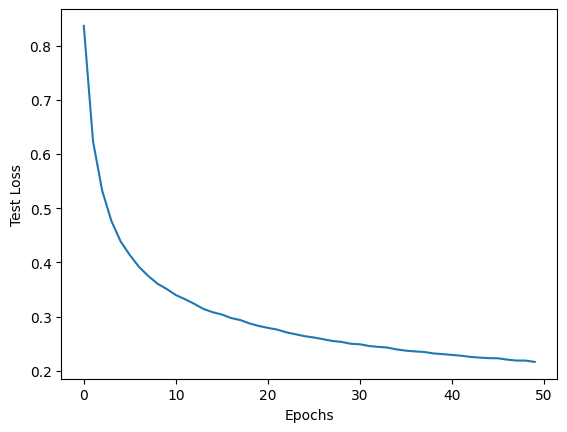
\includegraphics[scale=0.5]{Images/32_0.01.png}
        \end{figure}

        $\alpha=0.001$, epochs=50, batchsize=32\\
        Test Error: 13.76\%, Loss: 0.45
        \begin{figure}[H]
            \centering
            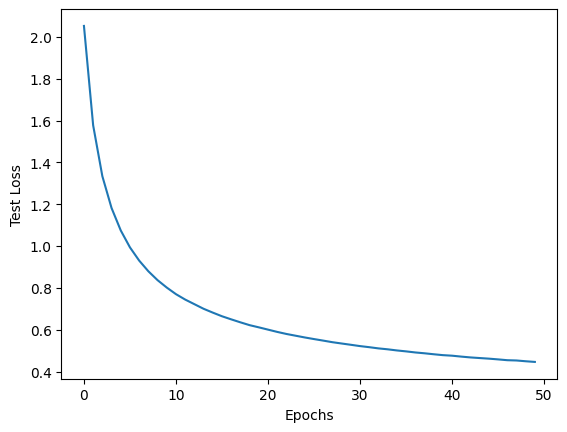
\includegraphics[scale=0.5]{Images/32_0.001.png}
        \end{figure}

        $\alpha=0.001$, epochs=50, batchsize=64\\
        Test Error: 17.50\%, Loss: 0.56
        \begin{figure}[H]
            \centering
            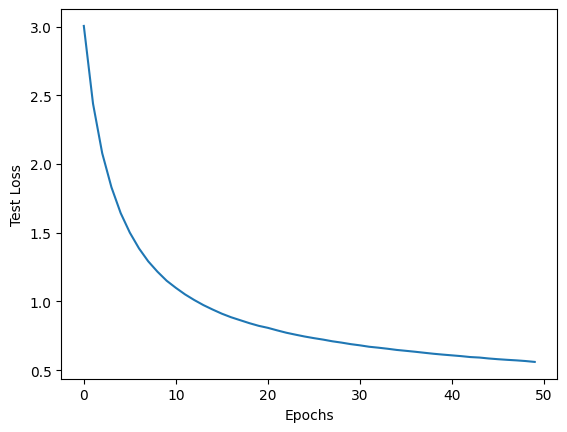
\includegraphics[scale=0.5]{Images/64_0.001.png}
        \end{figure}
    \end{soln}
    \item Implement the same network in PyTorch (or any other framework). You can use all the features of the framework e.g. auto-grad etc. Evaluate it on MNIST dataset, report test errors, and learning curve. (2 pts)
    \begin{soln}
        $\alpha=0.01$, epochs=50, batchsize=32\\
        Test Error: 6.68\%, Train Loss: 0.15
        \begin{figure}[H]
            \centering
            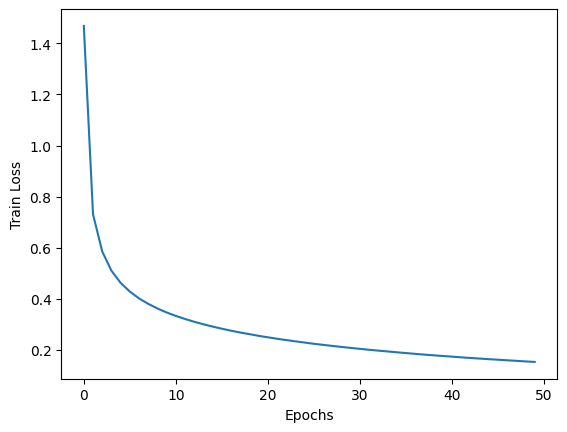
\includegraphics[scale=0.5]{Images/py_32_0.01.png}
        \end{figure}

        $\alpha=0.001$, epochs=50, batchsize=32\\
        Test Error: 13.95\%, Train Loss: 0.45
        \begin{figure}[H]
            \centering
            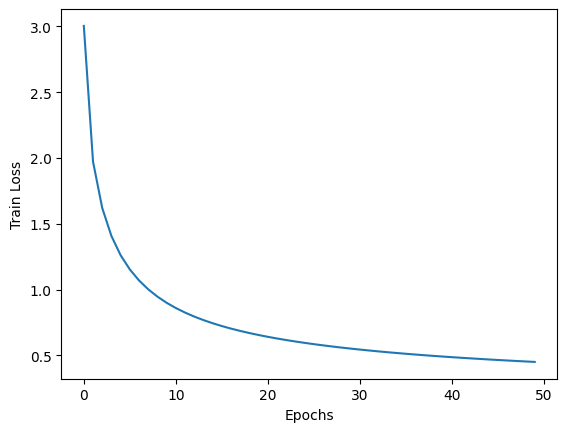
\includegraphics[scale=0.5]{Images/py_32_0.001.png}
        \end{figure}

        $\alpha=0.01$, epochs=50, batchsize=64\\
        Test Error: 8.76\%, Loss: 0.22
        \begin{figure}[H]
            \centering
            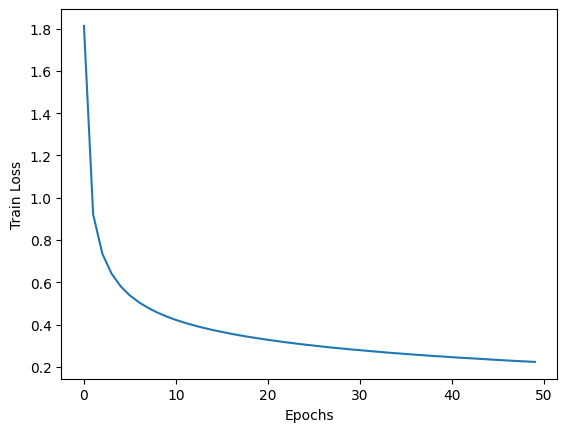
\includegraphics[scale=0.5]{Images/py_64_0.01.png}
        \end{figure}
    \end{soln}
    \item Try different weight initialization a) all weights initialized to 0, and b) initialize the weights randomly between -1 and 1. Report test error and learning curves for both. (You can use either of the implementations) (3 pts)
    
    \begin{soln}
        With weights Initialized with zeros.\\
        $\alpha=0.01$, epochs=50, batchsize=32\\
        Test Error: 22.26\%, Train Loss: 0.76
        \begin{figure}[H]
            \centering
            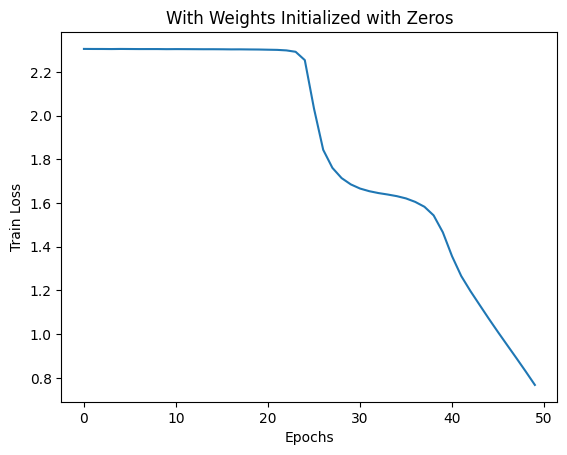
\includegraphics[scale=0.5]{Images/zero_init.png}
        \end{figure}

        With weights initialized with uniform distribution between -1 and 1.\\
        $\alpha=0.01$, epochs=50, batchsize=32\\
        Test Error: 7.06\%, Train Loss: 0.158
        \begin{figure}[H]
            \centering
            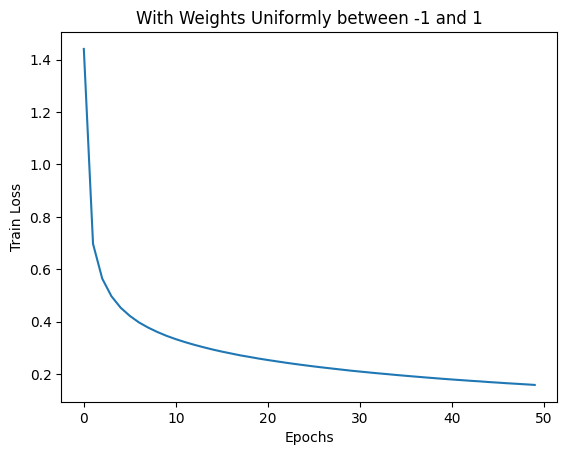
\includegraphics[scale=0.5]{Images/uniform_init.png}
        \end{figure}
    \end{soln}
\end{enumerate}

You should play with different hyperparameters like learning rate, batch size, etc. for your own learning. You only need to report results for any particular setting of hyperparameters. You should mention the values of those along with the results. Use $d_1 = 300$, $d_2 = 200$, $d_3 = 100$. For optimization use SGD (Stochastic gradient descent) without momentum, with some batch size say 32, 64, etc. MNIST can be obtained from here (https://pytorch.org/vision/ stable/datasets.html)

\bibliographystyle{apalike}
\end{document}
